
\nomenclature{FPGA}{Field-Programmable Gate Array}
\nomenclature{PWM}{Pulse Width Modulation}


\chapter{Preliminary analysis}
The system will consist of four parts overall. As shown in figure \ref{fig:firstsystem}, the physical system is connected with an FPGA, which is connected with SPI to a microprocessor,  which is then connected to I/O devices.

\begin{figure}[htb]
\centering
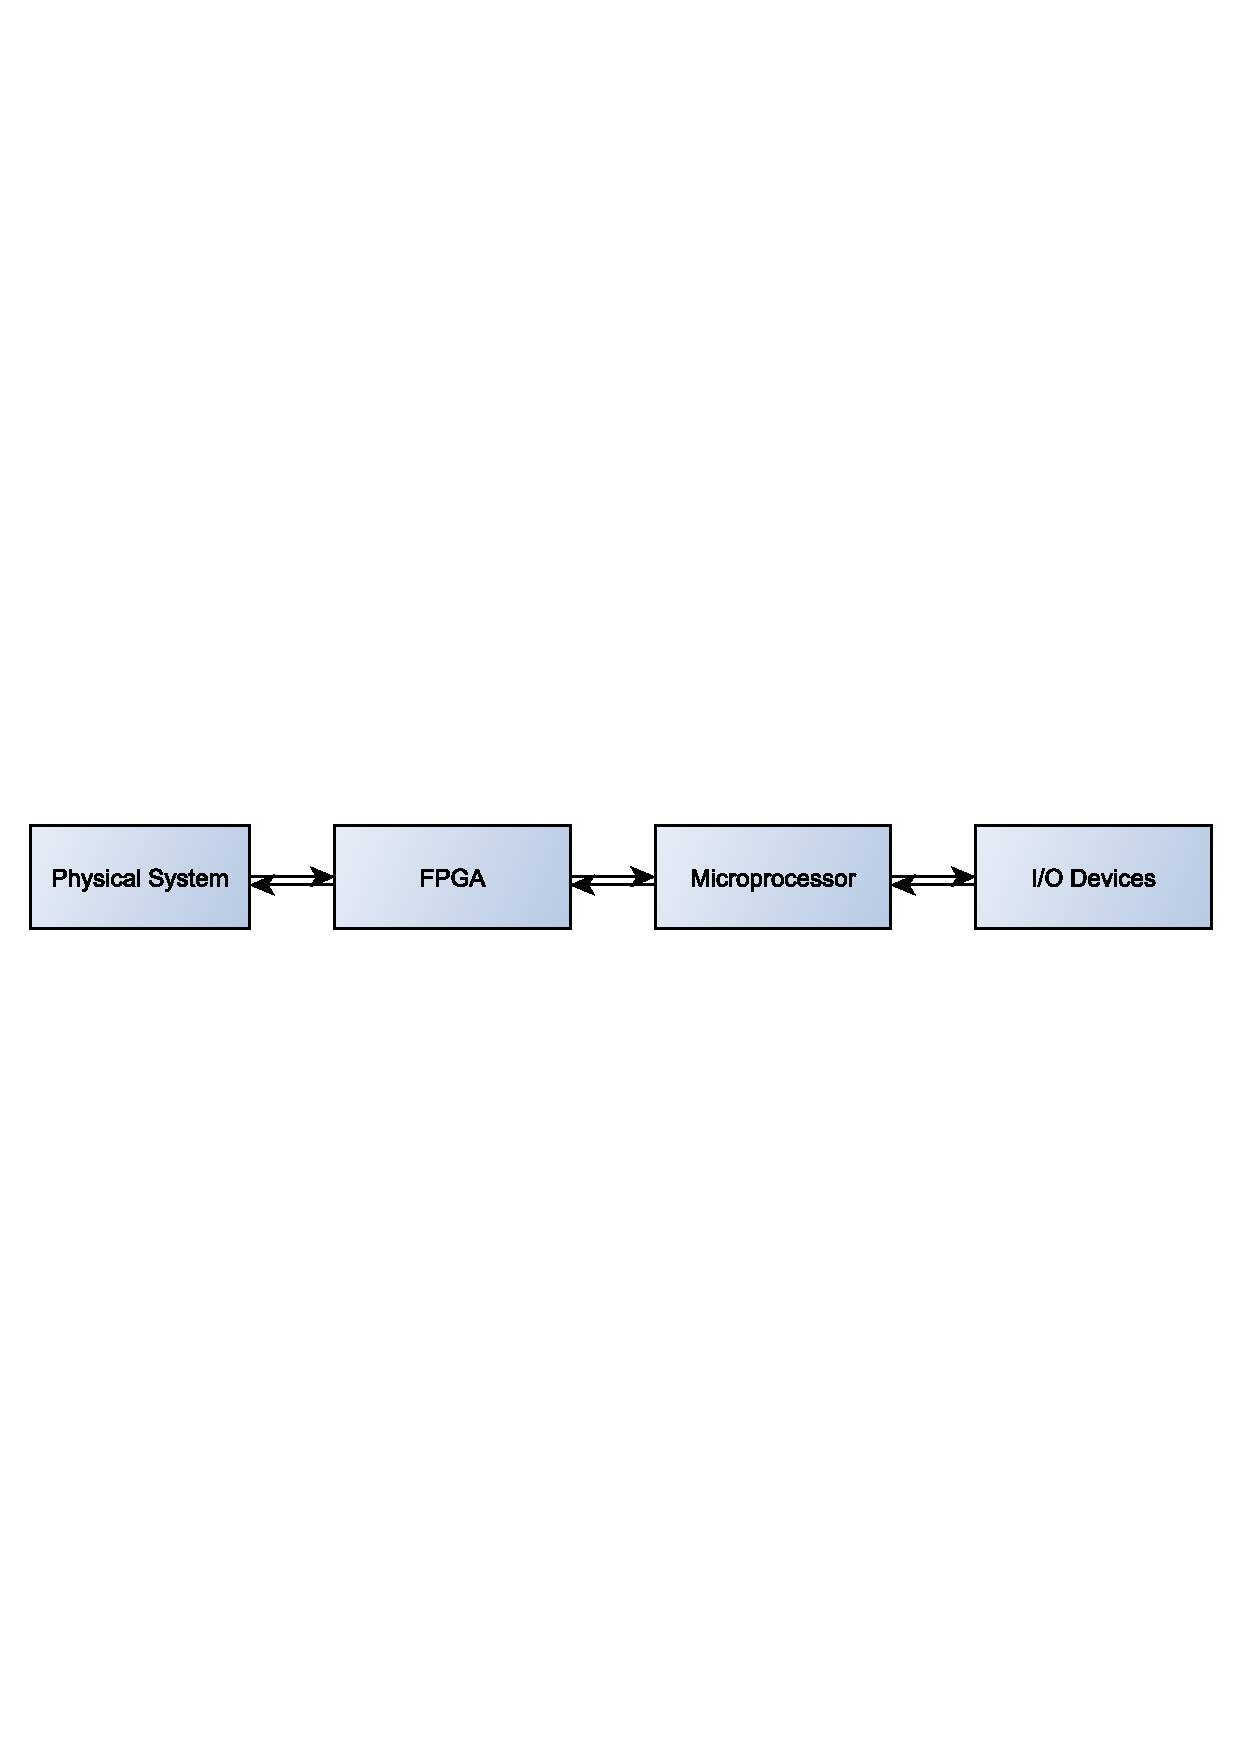
\includegraphics[scale=0.56,trim=400 380 400 380]{graphics/firstsystem.pdf} %trim=l b r t
\caption{Overall view of the system.}
\label{fig:firstsystem}	
\end{figure}

\section{The physical system}\label{sec:physicalsystem}
The physical system provided for the project consist of a pan/tilt system driven by two EMG30 \cite{emg30} motors with built-in encoders. The motors are driven by an H-bridge \cite{hbridge} with 12 volt DC supply connected. The system is controlled trough the H-bridge and output is collected by the encoders.

\begin{figure}[htb]
	\centering
	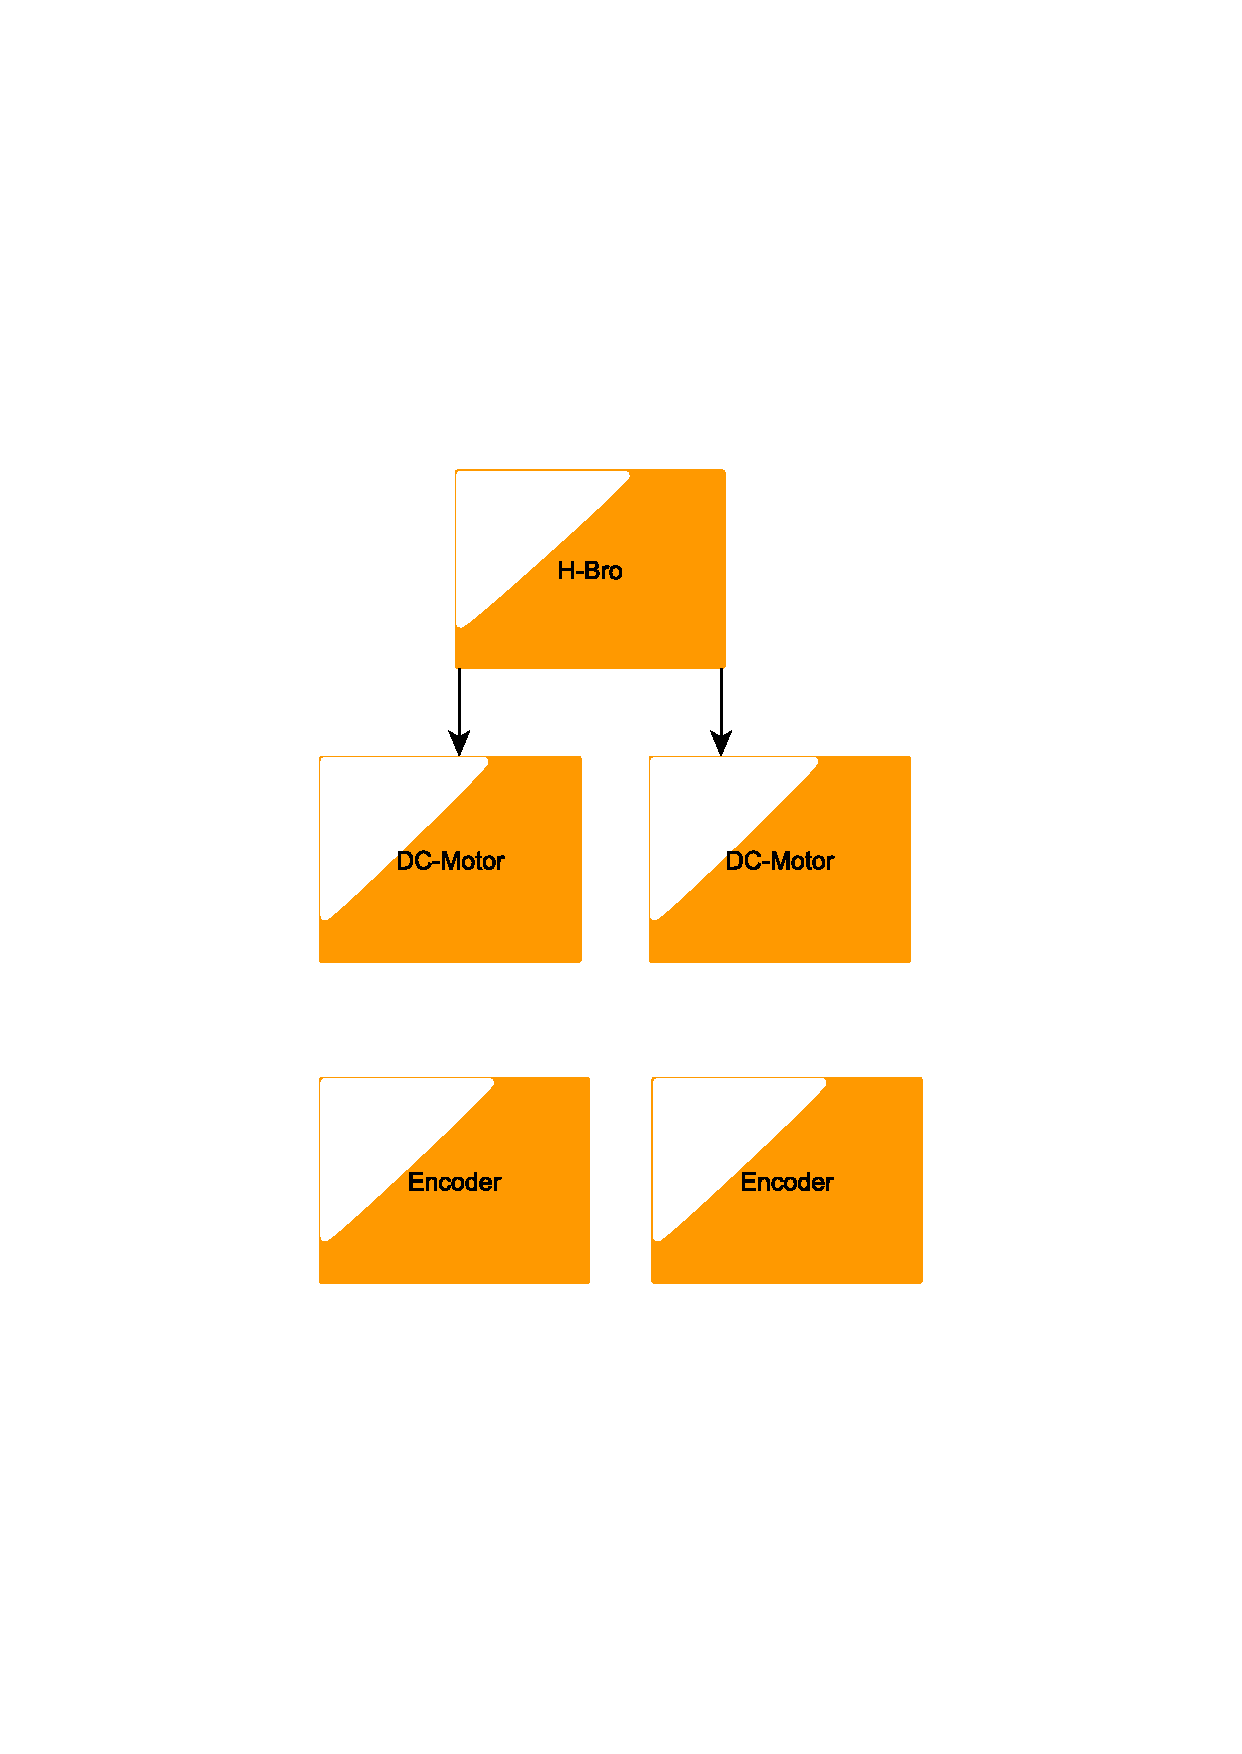
\includegraphics[scale=0.42,trim=200 200 200 200]{graphics/phsycicalsystem} %trim=l b r t (can cut off from every side)
	\caption{Set up of the physical system.}
	\label{fig:phsysicalsystem}			% figure labels are of the form \label{fig:*}
\end{figure}

\section{FPGA system}\label{sec:FPGA}

The FPGA is a Xilinx Nexys 2 board with a Spartan-3E chip on board \cite{nexys2}. Multiple processes will have to run on the FPGA. It is controlling the motors, watching the encoders and communicating with the microprocessor. The three main processes are the SPI communication, the motor PWM and the encoder. Both the PWM and encoder process are to run double because two motors are controlled. 

\begin{figure}[htb]
	\centering
	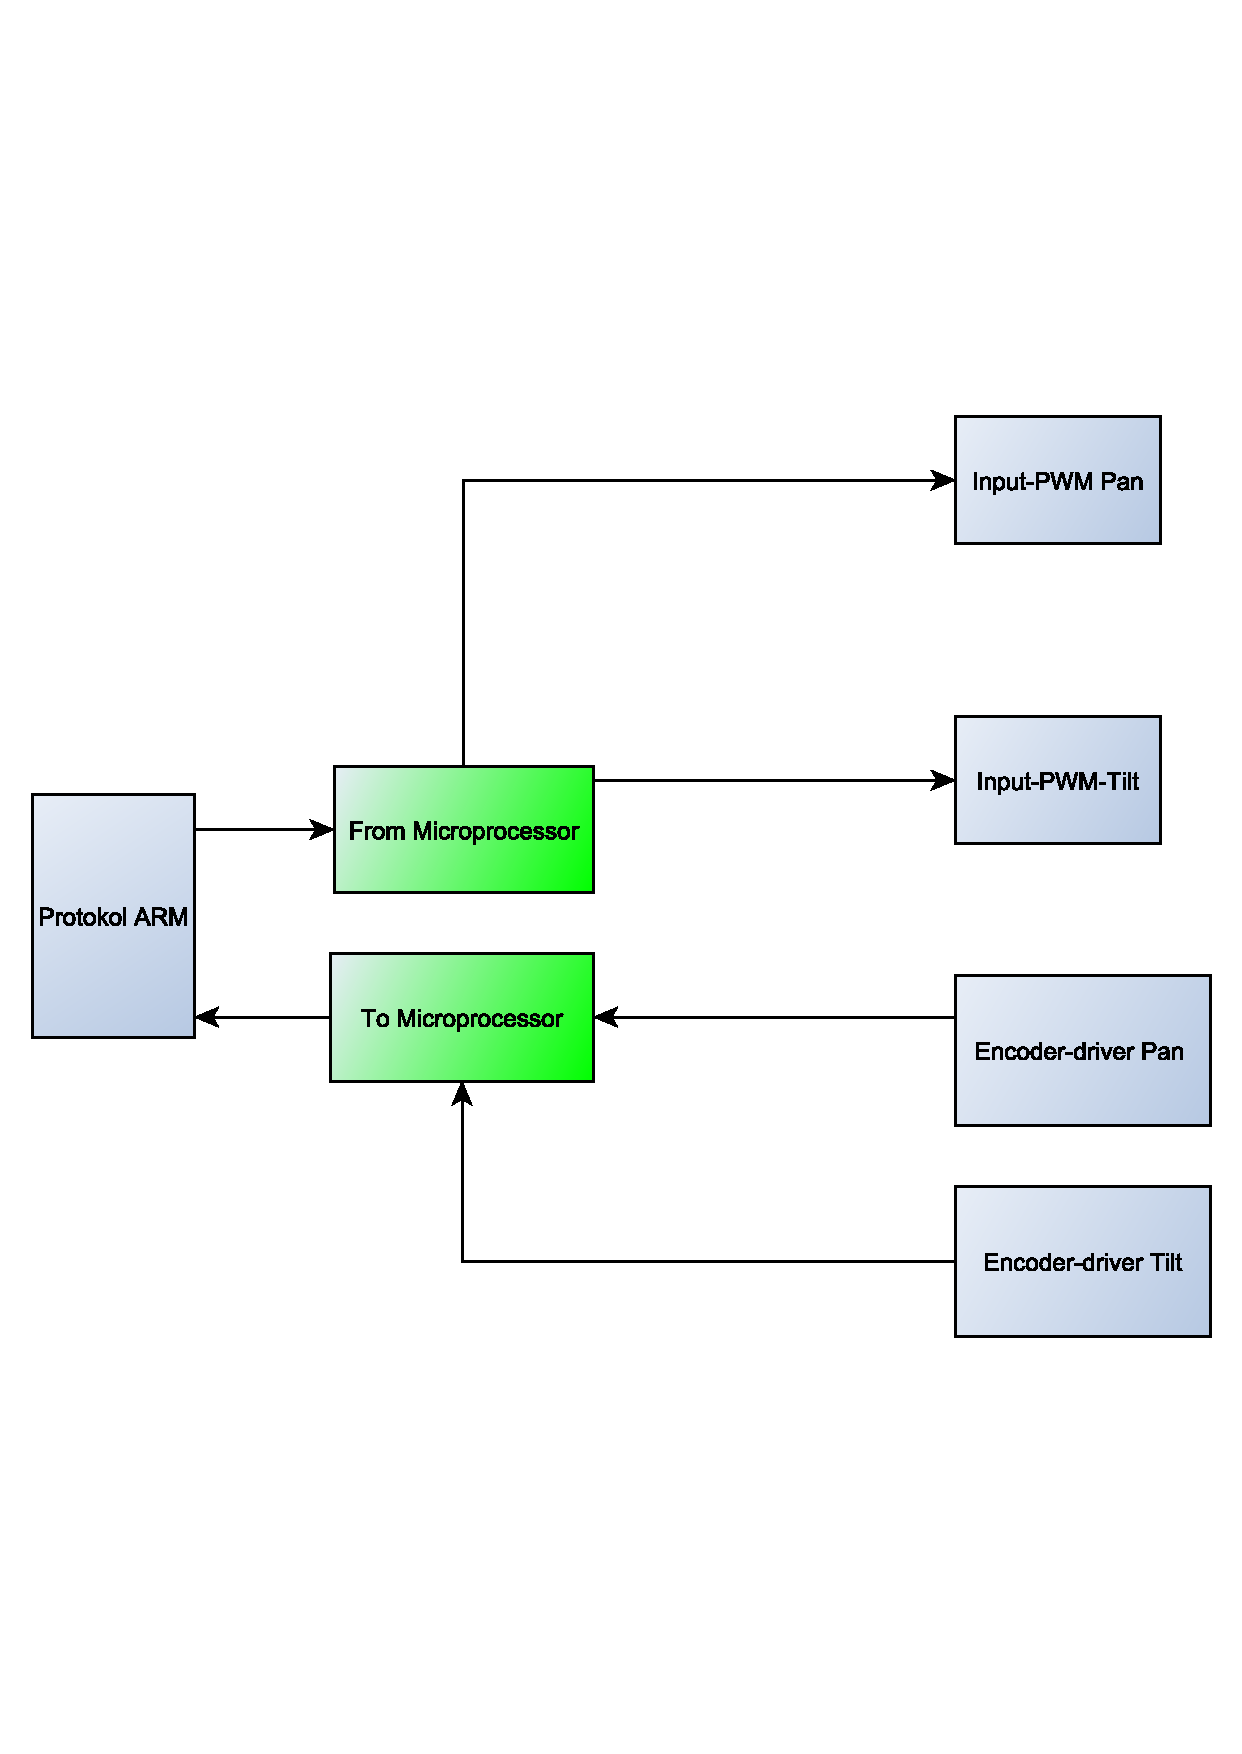
\includegraphics[scale=0.42,trim=200 200 200 200]{graphics/FPGA} %trim=l b r t (can cut off from every side)
	\caption{Setup of the FPGA processes.}
	\label{fig:FPGA}			% figure labels are of the form \label{fig:*}
\end{figure}

\section{Microprocessor}\label{sec:microprocessor}

The microprocessor is a LM3S6965 \cite{lm3s6965}, which implements an ARM Cortex-M3 core \cite{cm3}, mounted on a Stellaris evaluation board \cite{evalboard}. The microprocessor both runs the \hyperref[chap:control_system]{control}, the \hyperref[chap:ui]{user interface} and the \hyperref[sec:armspi]{communication through the SPI}. Parameters defining motor position, current PWM values and so forth are shared between each module ensuring a common interface between them. These parameters are listed in table \ref{tab:parameters}. Because the microprocessor will run multiple tasks communicating with each other, some sort of \hyperref[chap:os]{scheduler and intertask communication} will be needed. All these things will be discussed in detail in the coming chapters.

\begin{figure}[htb]
	\centering
	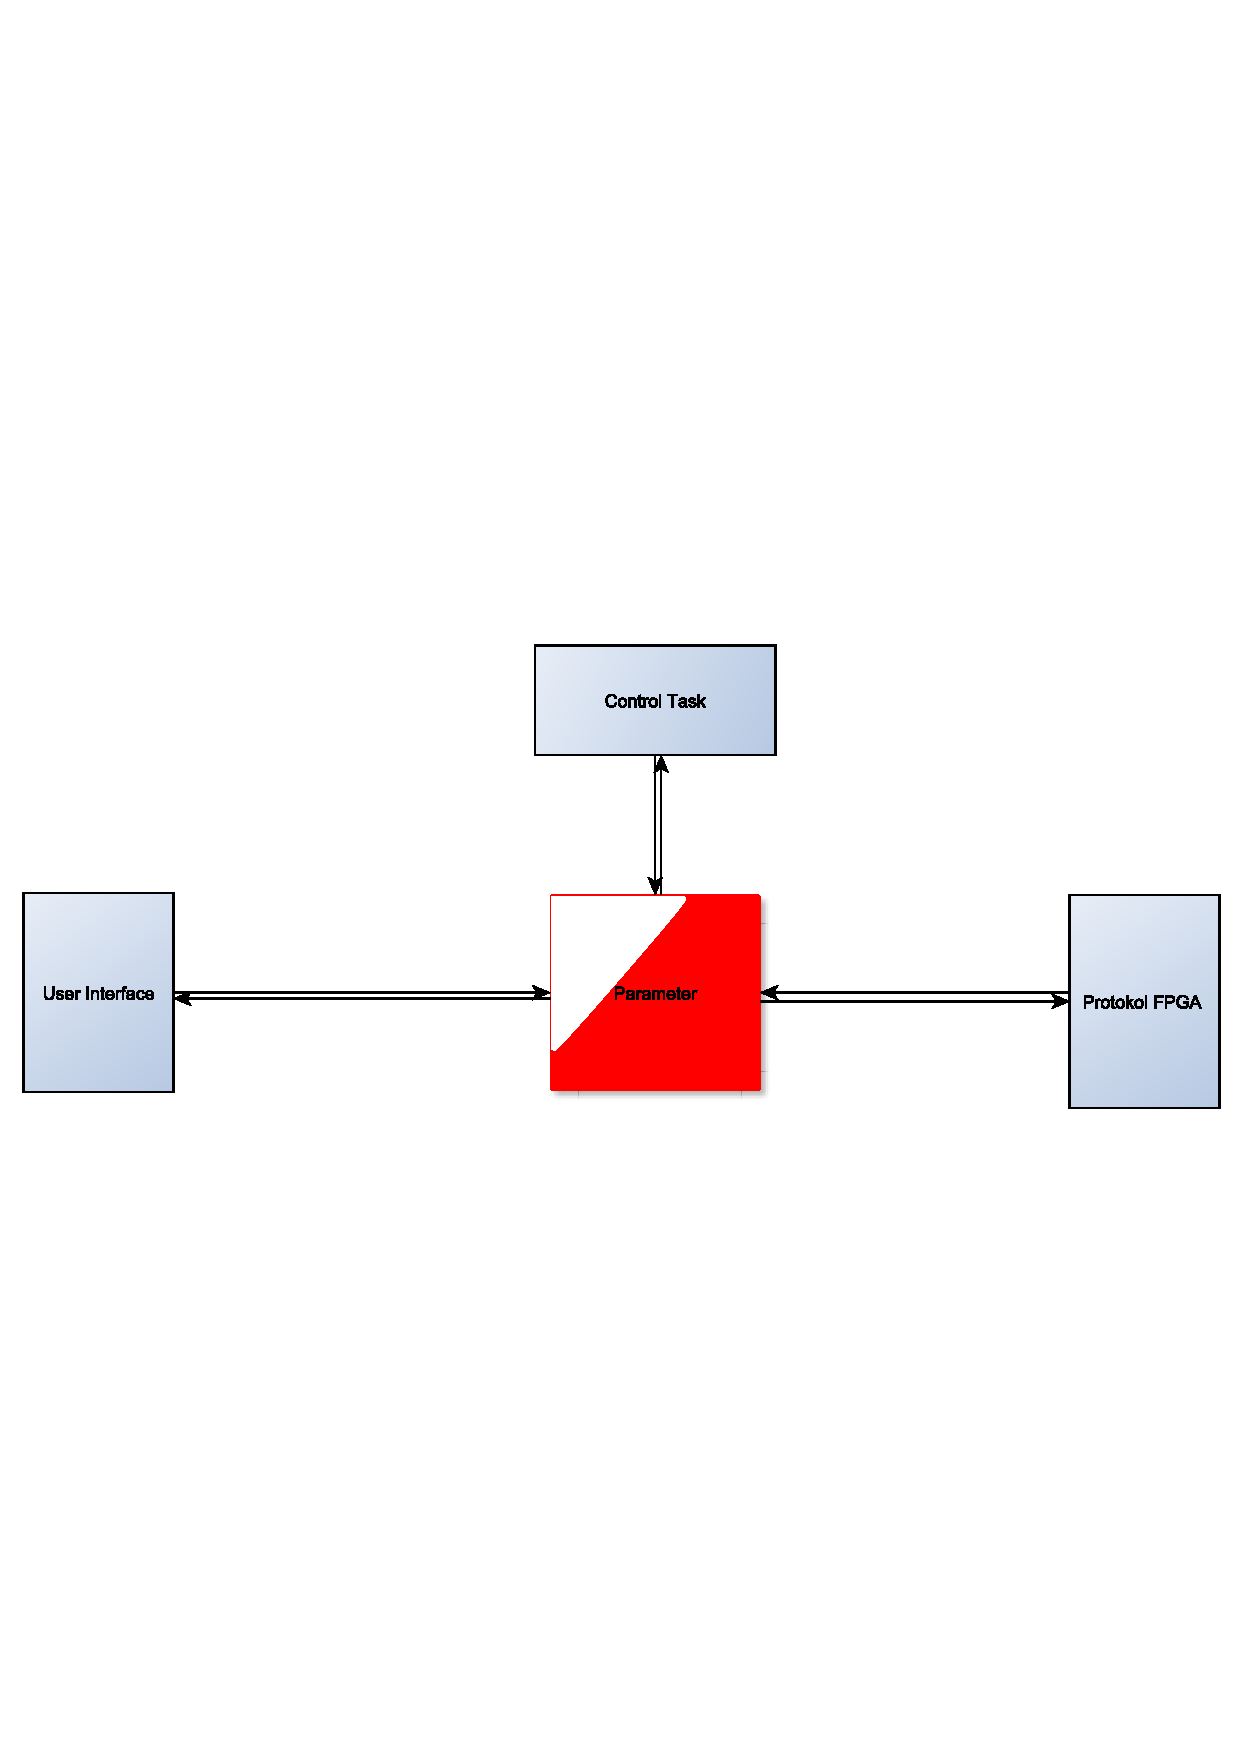
\includegraphics[scale=0.58,clip,trim=0 300 0 300]{graphics/microprocessor} %trim=l b r t (can cut off from every side)
	\caption{A simplified diagram of the microprocessor software modules.}
	\label{fig:microprocessor}			% figure labels are of the form \label{fig:*}
\end{figure}


\begin{table}[htb]				
	\centering
	\begin{tabular}{llccccc}			
	Parameter & Format & Unit & ARM & FPGA & Min value & Max value\\		
	\midrule										
Pan PWM  &16 bit signed & none & r/w & r & -32767 &  32768  \\
Tilt PWM  & 16 bit signed  & none&r/w & r & -32767 &  32768 \\
Pan position & 16 bit unsigned&ticks & r & w & 32544 & 32976 \\
Tilt position & 16 bit unsigned&ticks & r & w & 0 & 65535 \\
Pan velocity  & 16 bit unsigned&ticks/s & r & w & 0 & 65535 \\
Tilt velocity  & 16 bit unsigned & ticks/s&r & w & 0 & 65535 \\
Aux  & 16 bit unsigned &binary& r/w & r/w & 0 & 65535 \\
Pan current & 32 bit signed & 1/10 deg & r/w & - & -900 & 900 \\
Tilt current  & 32 bit signed & 1/10 deg & r/w & - & -109441 & 109441 \\
Pan setpoint  & 32 bit signed & 1/10 deg & r/w & - & -900 & 900 \\
Tilt setpoint  & 32 bit signed & 1/10 deg & r/w & - & -109441 & 109441 \\
	\end{tabular}
	\caption{Parameters that define the system.}				
	\label{tab:parameters}			
\end{table}


\section{I/O devices}\label{sec:iodevices}
When the microprocessor evaluation board was provided, an additional test board, incorporating more I/O peripherals, was included. The I/O devices should make it possible to input data to, and receive output from, the control system easily. There are two LCD's usable as output and a numeric keypad, buttons, an incremental rotary encoder and a potentiometer as possible inputs.
%Thus the incremental rotary encoder is chosen as main input to avoid many different %inputs, though the numpad is also included for situations were the incremental %encoder cannot be used. The test boards LCD was chosen because it is bigger and %therefore it can easier show feedback.
\begin{figure}[htb]
	\centering
	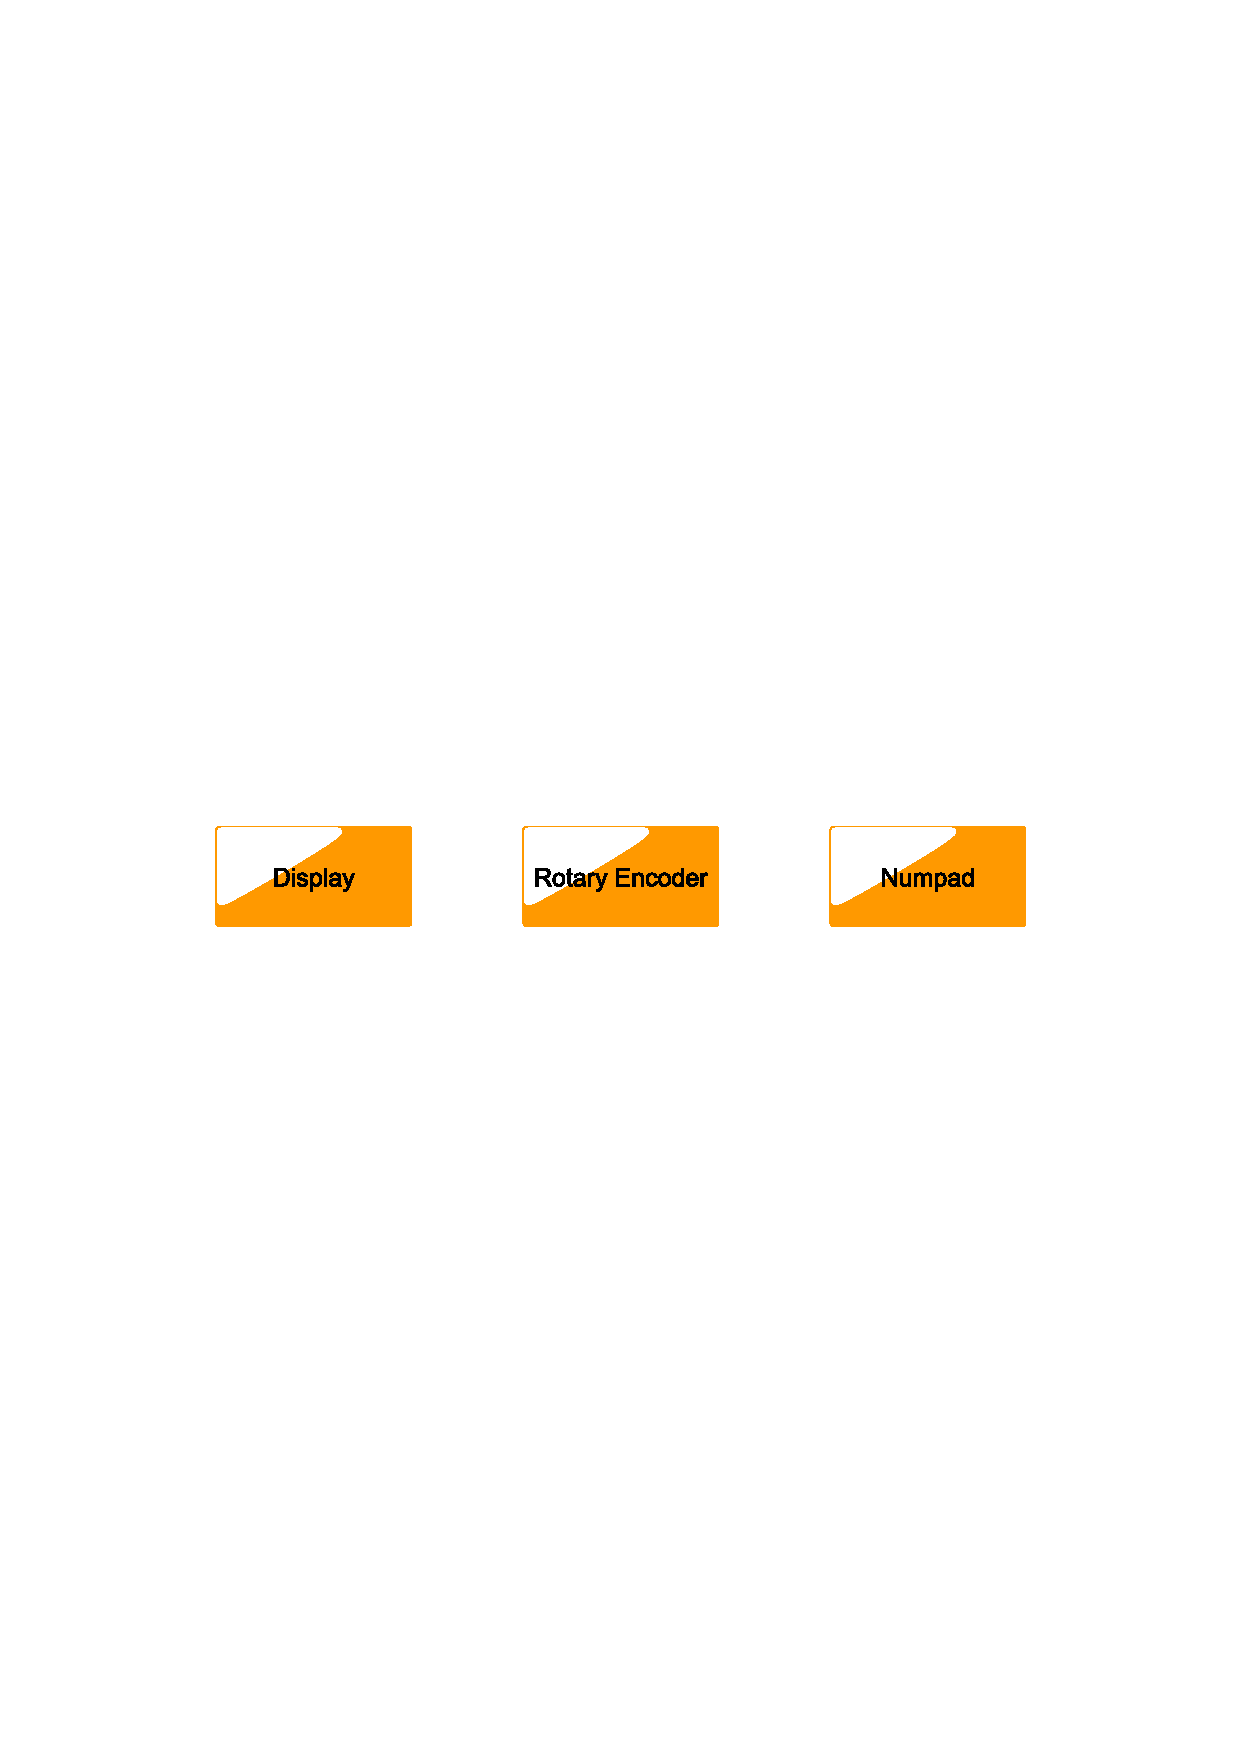
\includegraphics[scale=0.6,clip,trim=00 400 00 400]{graphics/iodevices} %trim=l b r t (can cut off from every side)
	\caption{Set up of the I/O devices.}
	\label{fig:iodevices}			% figure labels are of the form \label{fig:*}
\end{figure}


\section{The complete system}

The electrical system was set up as shown in figure \ref{fig:digitalsystem}. All the user interface in- and outputs are mounted with the microprocessor, all the motor in- and output at the FPGA, and a SPI connection between the two.

\begin{figure}[htb]
	\centering
	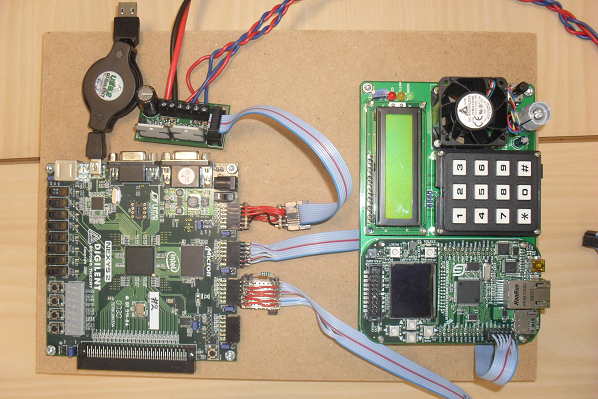
\includegraphics[width=\textwidth]{graphics/digitalsystem.png} %trim=l b r t (can cut off from every side)
	\caption{Set up of the electrical system.}
	\label{fig:digitalsystem}			% figure labels are of the form \label{fig:*}
\end{figure}


The complete system is shown in figure \ref{fig:completesystem}, this shows the parts the system have been divided into. This is not meant to show the exact number of tasks, but as a reference to understand the components in the system.


\begin{figure}[htb]
	\centering
	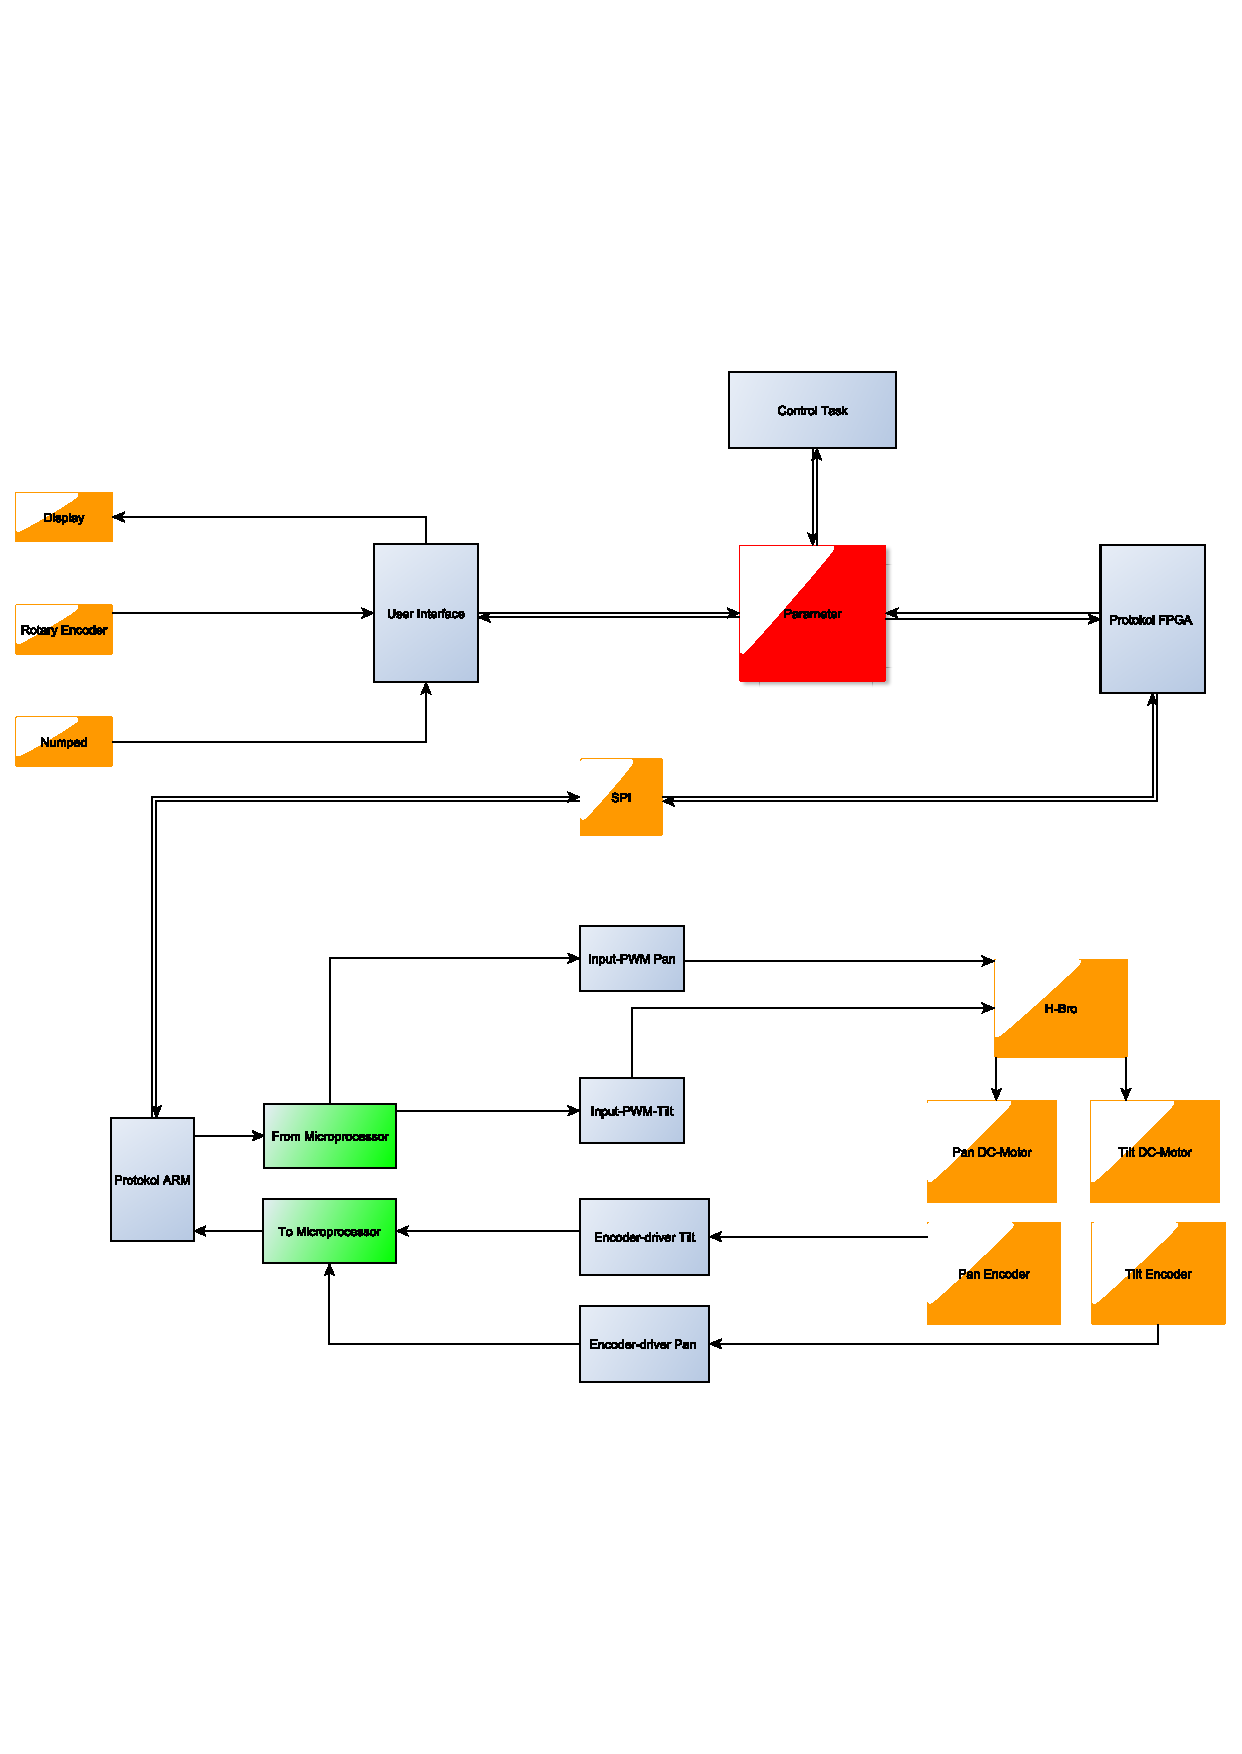
\includegraphics[width=\textwidth,clip,trim=0 160 0 160]{graphics/Project4GreaterPresentation4.pdf} %trim=l b r t 
	\caption{The combined model of parts that the system will consist of. }
	\label{fig:completesystem}			% figure labels are of the form \label{fig:*}
\end{figure}
